%%%%%%%%%%%%%%%%%%%%%%%%%%%%%%%%%%%%%%%%%
% baposter Landscape Poster
% LaTeX Template
% Version 1.0 (11/06/13)
%
% baposter Class Created by:
% Brian Amberg (baposter@brian-amberg.de)
%
% This template has been downloaded from:
% http://www.LaTeXTemplates.com
%
% License:
% CC BY-NC-SA 3.0 (http://creativecommons.org/licenses/by-nc-sa/3.0/)
%
%%%%%%%%%%%%%%%%%%%%%%%%%%%%%%%%%%%%%%%%%

%----------------------------------------------------------------------------------------
%	PACKAGES AND OTHER DOCUMENT CONFIGURATIONS
%----------------------------------------------------------------------------------------

\documentclass[landscape,a0paper,fontscale=0.285]{baposter} % Adjust the font scale/size here
\usepackage{url}
\usepackage{bm}
\usepackage{graphicx} % Required for including images
\graphicspath{{figures/}} % Directory in which figures are stored
\usepackage{ragged2e}
\usepackage{amsmath} % For typesetting math
\usepackage{amssymb} % Adds new symbols to be used in math mode

\usepackage{booktabs} % Top and bottom rules for tables
\usepackage{enumitem} % Used to reduce itemize/enumerate spacing
\usepackage{palatino} % Use the Palatino font
\usepackage[font=small,labelfont=bf]{caption} % Required for specifying captions to tables and figures

\usepackage{multicol} % Required for multiple columns
\setlength{\columnsep}{1.5em} % Slightly increase the space between columns
\setlength{\columnseprule}{0mm} % No horizontal rule between columns

\usepackage{tikz} % Required for flow chart
\usetikzlibrary{shapes,arrows} % Tikz libraries required for the flow chart in the template

\newcommand{\compresslist}{ % Define a command to reduce spacing within itemize/enumerate environments, this is used right after \begin{itemize} or \begin{enumerate}
\setlength{\itemsep}{1pt}
\setlength{\parskip}{0pt}
\setlength{\parsep}{0pt}
}

\definecolor{lightgray}{rgb}{.85,.85,.85} % Defines the color used for content box headers
\definecolor{carrotorange}{rgb}{0.93, 0.57, 0.13}

\begin{document}

\begin{poster}
{
headerborder=closed, % Adds a border around the header of content boxes
colspacing=1em, % Column spacing
bgColorOne=lightgray, % Background color for the gradient on the left side of the poster
bgColorTwo=lightgray, % Background color for the gradient on the right side of the poster
borderColor=black, % Border color
headerColorOne=orange, % Background color for the header in the content boxes (left side)
headerColorTwo=carrotorange, % Background color for the header in the content boxes (right side)
headerFontColor=black, % Text color for the header text in the content boxes
boxColorOne=white, % Background color of the content boxes
textborder=roundedleft, % Format of the border around content boxes, can be: none, bars, coils, triangles, rectangle, rounded, roundedsmall, roundedright or faded
eyecatcher=true, % Set to false for ignoring the left logo in the title and move the title left
headerheight=0.1\textheight, % Height of the header
headershape=roundedright, % Specify the rounded corner in the content box headers, can be: rectangle, small-rounded, roundedright, roundedleft or rounded
headerfont=\Large\bf\textsc, % Large, bold and sans serif font in the headers of content boxes
%textfont={\setlength{\parindent}{1.5em}}, % Uncomment for paragraph indentation
linewidth=2pt % Width of the border lines around content boxes
}
%----------------------------------------------------------------------------------------
%	TITLE SECTION 
%----------------------------------------------------------------------------------------
%
{
\includegraphics[height=4em]{PS_HOR_RGB_2C.png}} % First university/lab logo on the left
{\bf\textsc{The Network of Foreign Direct Investment Flows}\vspace{0.5em}} % Poster title
{\textsc{John Schoeneman, Boliang Zhu, \& Bruce Desmarais\\
Pennsylvania State University}} % Author names and institution
{
{\includegraphics[height=4em]{nsf.png}} % Second nsf logo on the right
{
\includegraphics[height=4em]{bdss.png}}
}
%----------------------------------------------------------------------------------------
%	introduction
%----------------------------------------------------------------------------------------

\headerbox{Introduction}{name=introduction,column=0,row=0}{
\begin{itemize}[leftmargin=*, nolistsep]

\item While substantial work has been done investigating exogenous political and economic determinants of FDI flows, most existing studies of the political economy of FDI overlook the complex dependencies that are likely to characterize the network. \\

\item In this paper, we integrate hypotheses regarding exogenous determinants and novel hypotheses regarding structural dependencies into a comprehensive exponential random graph model (ERGM) for weighted networks.$^1$
\end{itemize}
\vspace{1em} % When there are two boxes, some whitespace may need to be added if the one on the right has more content
}



%----------------------------------------------------------------------------------------
%	RESULTS
%----------------------------------------------------------------------------------------

\headerbox{Select Results}{name=results,column=1,span=2,row=0}{

\centering
\begin{tabular}{c@{\hskip -.1cm}c@{\hskip -.1cm}c@{\hskip -.1cm}}
Log-GDP Product & Distance  & PTA Depth  \\
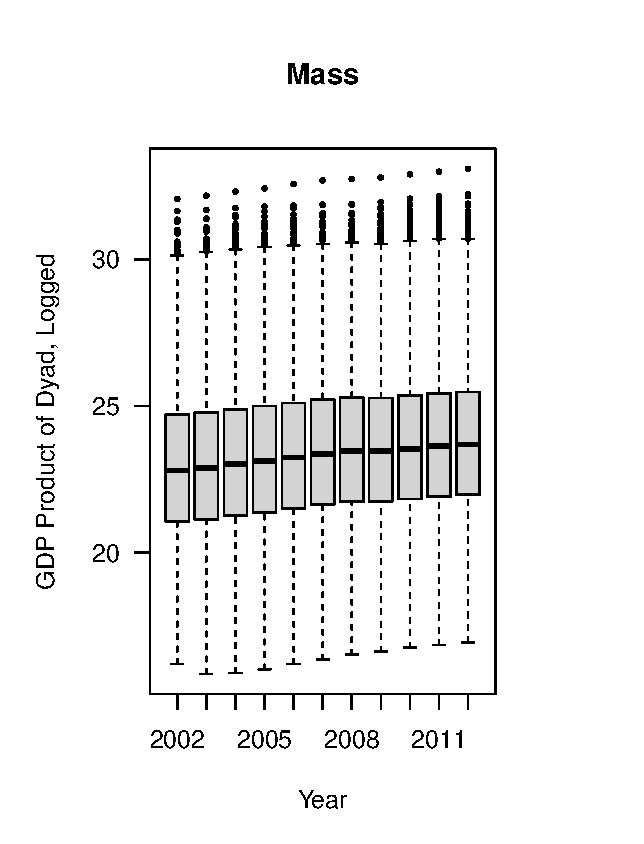
\includegraphics[height=.14\textheight, clip=true, trim=.5cm .4cm 0cm .1cm]{figures/rl_plots/mass.pdf}    &
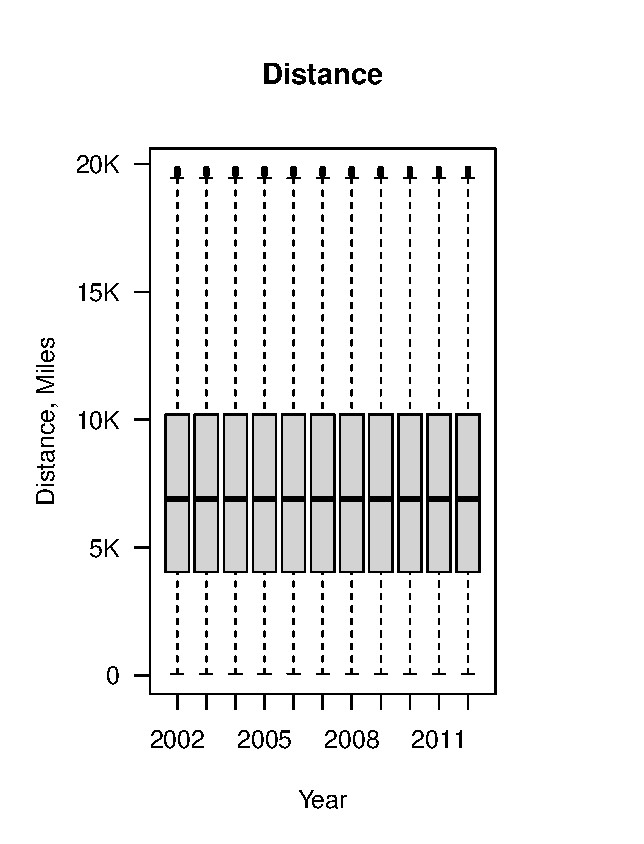
\includegraphics[height=.14\textheight, clip=true, trim=.5cm .4cm 0cm .1cm]{figures/rl_plots/distance.pdf}   &
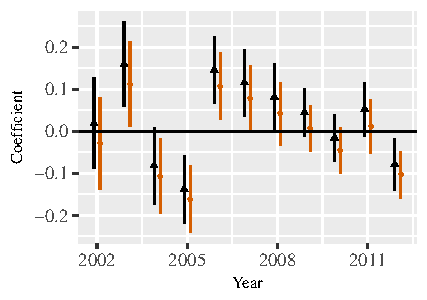
\includegraphics[height=.14\textheight, clip=true, trim=.5cm .4cm 0cm .1cm]{figures/rl_plots/PTADepth.pdf}\\


Destination Polity & Reciprocity & Transitivity \\ 
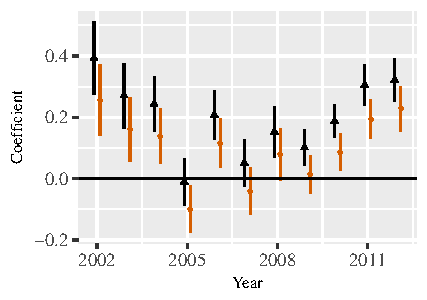
\includegraphics[height=.14\textheight, clip=true, trim=.5cm .5cm 0cm .1cm]{figures/rl_plots/DestPolity.pdf} 
 &
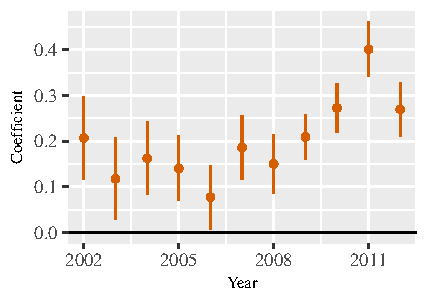
\includegraphics[height=.14\textheight, clip=true, trim=.5cm .5cm 0cm .1cm]{figures/rl_plots/Mutuality.pdf}   &
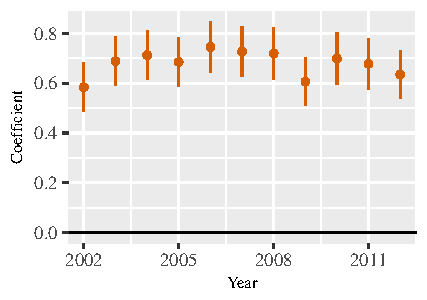
\includegraphics[height=.14\textheight, clip=true, trim=.5cm .5cm 0cm .1cm]{figures/rl_plots/Transitivity.pdf} \\  
\end{tabular}
\vfill
Bars represents 95\% Confidence intervals. Black triangles are coefficient estimates without controlling for network dependencies. Orange circles are estimates with network controls.

}

%----------------------------------------------------------------------------------------
% Data 
%----------------------------------------------------------------------------------------

\headerbox{Model Specification}{name=data,column=3,row=0}{ % This block's bottom aligns with the bottom of the conclusion block


%\begin{itemize}[leftmargin=4mm]\compresslist

%\item{Dependent Variable}\\
\centering{Box Plots of Non-Zero FDI Stocks}\\
%\end{itemize}
%\vspace*{-\baselineskip}
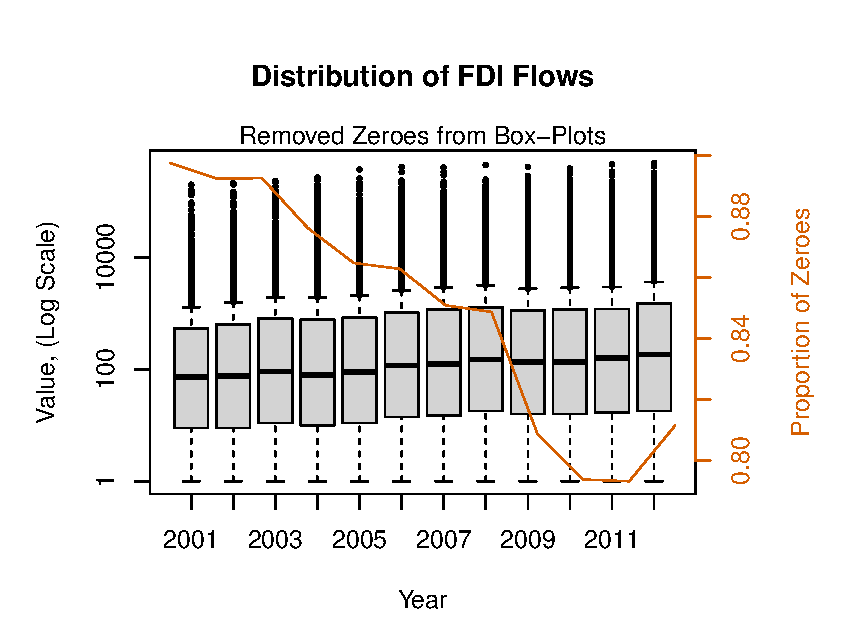
\includegraphics[scale=.58, clip=true, trim=.6cm 1.5cm .35cm 2cm]{figures/fdi_dist.pdf}
\vspace*{-\baselineskip}
\begin{itemize}[leftmargin=4mm]\compresslist
\item{Network Statistics}
\begin{itemize}
\item{Sum; Sum$^{1/2}$; Non-zero; Reciprocity; Transitive Weights}
\end{itemize}
\item{Dyad-level Covariates (expected)}
\begin{itemize}
\item{Gravity(+); Contiguity(+); Common Language(+); Four Types of Defense Treaties(+); Colonial Relationships(+); PTA depth(+)}
\end{itemize}
\item{Node-level Covariates (sender/receiver)}
\begin{itemize}
\item{GDP per capita(+/-); GDP Growth Rate(+/+); Polity IV(+/+); Political Violence(-/-); Trade Openness(+)}
\end{itemize}
\end{itemize}

%\textbf{Method}
%\begin{itemize}[leftmargin=4mm]\compresslist
%\item{Exponential Random Graph Model for Weighted Networks$^1$}
%\vspace{5mm}
%\end{itemize}


}

%----------------------------------------------------------------------------------------
%	Theory
%----------------------------------------------------------------------------------------

\headerbox{Dependence Hypotheses}{name=theory,column=0,below=introduction}{
\centering{

\Large{Reciprocity}\\
\normalsize{
\vspace{.4cm}
\hspace{0cm}$\sum_{(i,j) {\in} \mathbb{Y}}min(\bm{y}_{i,j},\bm{y}_{j,i})$
\vspace{.4cm}

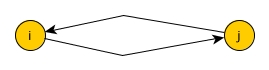
\includegraphics[height=.04\textheight, clip=true, trim=.5cm .5cm 0cm .1cm]{figures/reciprocity.jpg} \\  

\vspace{.4cm}
}
\Large{Transitivity}\\

\normalsize{
\vspace{.2cm}
\centering
$ \sum_{(i,j) {\in} \mathbb{Y}}\min\bigg( \bm{y}_{i,j}, \max\limits_{k{\in}N}\Big(\min(\bm{y}_{i,k},\bm{y}_{k,j})\Big) \bigg)$ 
\vspace{.4cm}


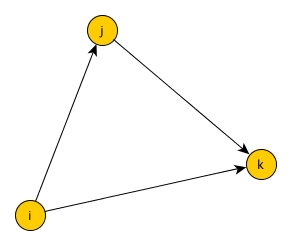
\includegraphics[height=.2\textheight, clip=true, trim=.5cm .5cm 0cm .1cm]{figures/transitivity.jpg} \\

\vspace{.4cm}  
}

}

}









%----------------------------------------------------------------------------------------
%	Network Plot
%----------------------------------------------------------------------------------------

\headerbox{Structural Dependency Plots}{name=network,column=1,span=2,row=0,below=results,above=references,bottomaligned=theory}{

\begin{multicols}{2}


Plot for 2011: Scale from Blue to red represents autocratic regimes to democratic regimes
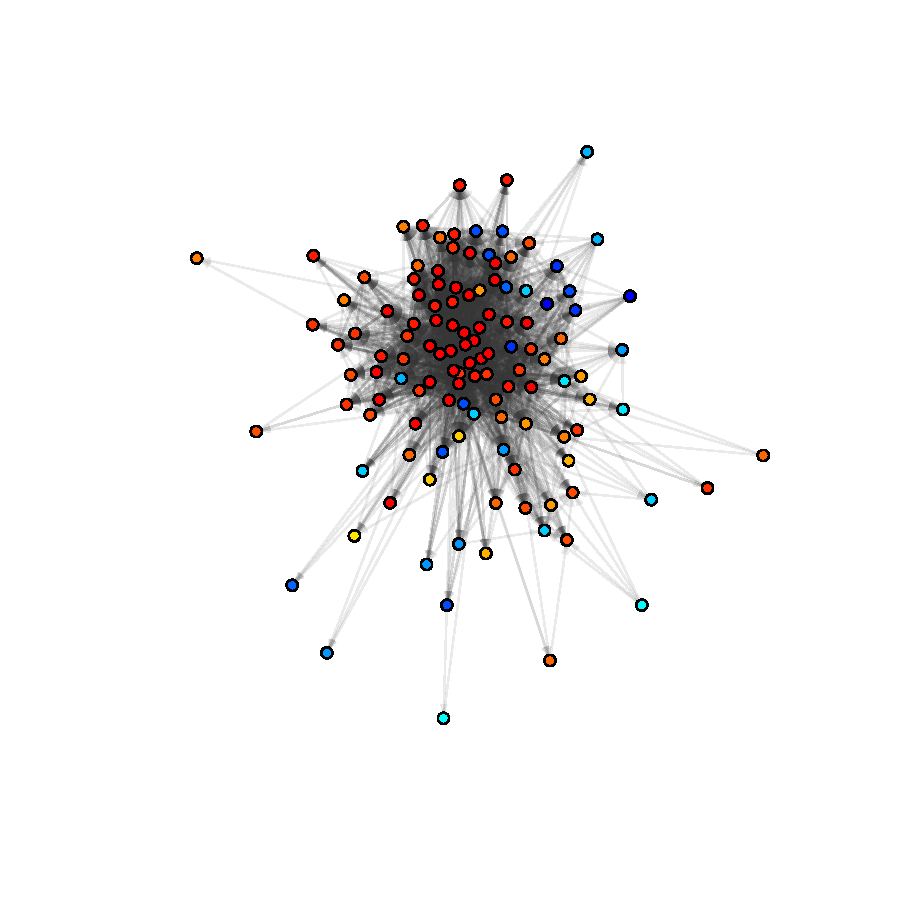
\includegraphics[scale=.6, clip=true, trim=2cm 0cm 0cm 2.3cm]{fdiNet2011.pdf}


%------------------------------------------------


\centering

\vfill{Reciprocity}
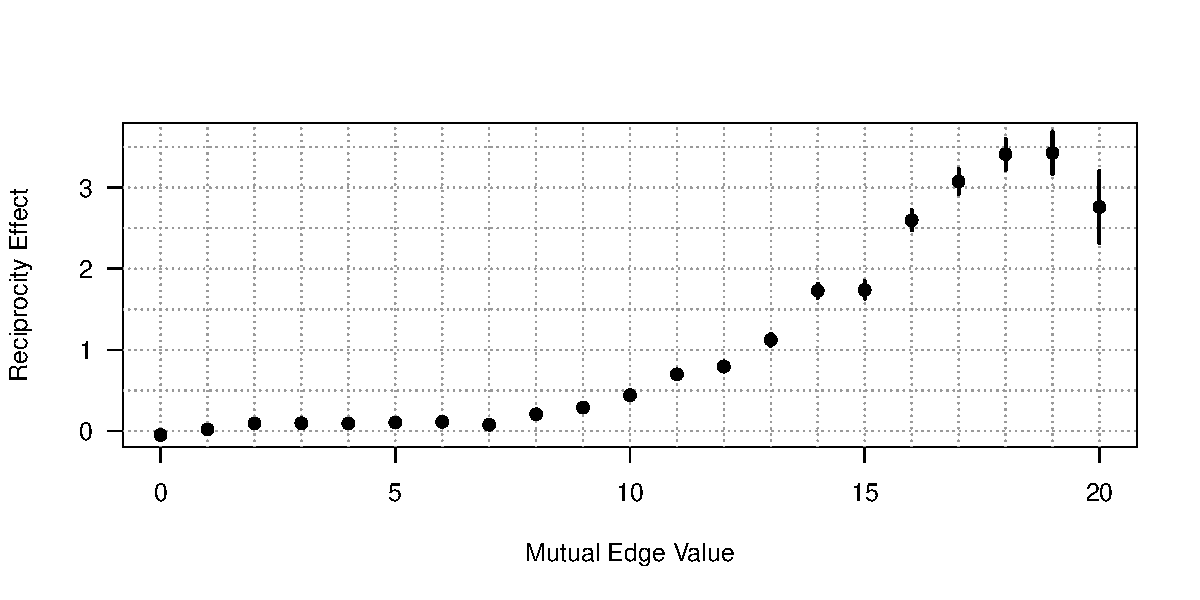
\includegraphics[scale=.4, clip=true, trim=1cm 1cm 0cm 1.5cm]{mutualInterpretation.pdf}
Transitivity
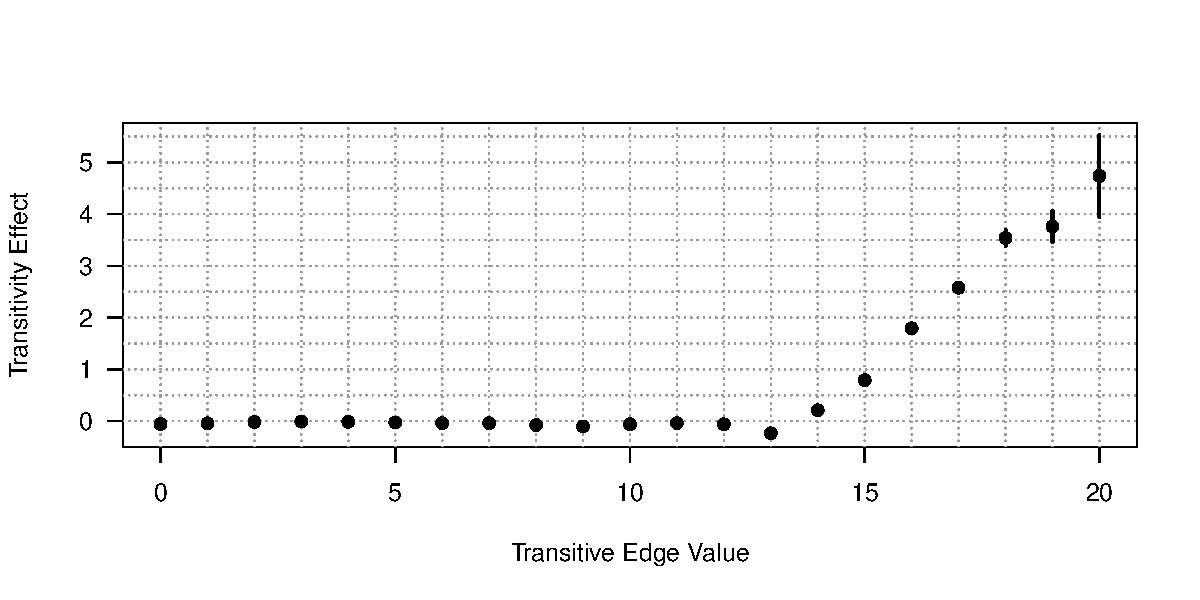
\includegraphics[scale=.4, clip=true, trim=1cm 1cm 0cm 1.5cm]{transitiveInterpretation.pdf}

\end{multicols}


}

%----------------------------------------------------------------------------------------
%	Results
%----------------------------------------------------------------------------------------

\headerbox{Discussion}{name=results2,column=3,below=data,bottomaligned=theory}{ 




\textbf{Inclusion of Network Dependency Terms:} 
\begin{itemize}[leftmargin=*, nolistsep]

\item For every year the model was fit, we saw a decrease in the BIC.

\item  The estimates of exogenous covariates shift opposite of the expected direction, moving from significant at the 95\% level to insignificant in some cases

\item The dependency terms are significant for every year. 

\item As the corresponding edge value(s) for structural dependency increase, models without structural terms become less accurate. 
\end{itemize}

\vspace{.2cm}



  

}

%----------------------------------------------------------------------------------------

%----------------------------------------------------------------------------------------
%	Acknowledgement
%----------------------------------------------------------------------------------------

\headerbox{Acknowledgement}{name=nsf,column=0,above=bottom}{

This material is based on work supported by the National Science Foundation under IGERT Grant DGE-1144860, Big Data Social Science.}

%----------------------------------------------------------------------------------------
%	REFERENCES
%----------------------------------------------------------------------------------------

\headerbox{Reference}{name=references,column=1,span=2,aligned=nsf,above=bottom}{ % This block is as tall as the references block


\small{1. Krivitsky, Pavel N. 2016. ergm.count: Fit, Simulate and Diagnose Exponential-Family Models for Networks with Count Edges. The Statnet Project (\texttt{http://www.statnet.org}). R package version 3.2.2.
\url{http://CRAN.R-project.org/package=ergm.count}}

}

%----------------------------------------------------------------------------------------
%	CONTACT INFORMATION
%----------------------------------------------------------------------------------------

\headerbox{Contact Information}{name=contact,column=3,aligned=nsf,above=bottom}{ % This block is as tall as the references block

\begin{description}\compresslist
\item[Department]  Political Science, Pond Labratory
\item[Web]  \url{github.com/desmarais-lab}
\item[Email] jbs5686@psu.edu
\end{description}
}


\end{poster}

\end{document}